\chapter{Teori}
I dette afsnit vil teorien, der ligger til grund for programmet, blive beskrevet, hvorunder tre hovedafsnit findes. Grafteori vil være det første afsnit, efterfulgt af vektorteori og  positionsbestemmelse. Under grafteori vil et par forskellige algoritmer tages i brug, hvoraf den bedste match til programmet findes. I grafteorien vil Nearest neighbor, Dijkstra’s algoritme og Double Minimum Spanning Tree algoritmerne blive beskrevet. I vektorteorien vil teorien bag udregning af afstanden mellem to knuder, eller en knude og en rute gøres rede for. Denne teori vil blive brugt i programmet til dannelse af rute, og udregning af nærliggende attraktioner.

\subsection{Grafteori}
Grafteori er et afsnit i denne rapport, som omhandler en generel forklaring på grafteori, hvorefter teorien bag Nearest neighbor algoritme, Dijkstra’s algoritme, Double Minimum Spanning Tree og Traveling salesman problem vil blive beskrevet. Alt dette beskrives, for at give et udgangspunkt for implementering af en hensigtsmæssig algoritme i programmet for denne rapport.\newline
Matematikken bag grafteori er ét aspekt af emnet, hvor visualisering og tegning er en anden. Den matematiske del behandler kombinationerne af knuder og kanter. En knude er et punkt, i dette tilfælde en attraktion, som skal besøges, hvor en kant er ruten mellem to knuder. En kant er derfor længden fra ét punkt til det næste \citep{GraphTheory}.
I grafteori er begrebet ”graf” mere fleksibelt, da punkterne ikke nødvendigvis har x, y eller z værdier, alt efter antallet af dimensioner det behandles i. Grafen er en afbildning af punkter i en form, der virker hensigtsmæssig. Heraf opstår isomorfe modeller, som er forskellige afbildninger, af selv samme graf. 

\begin{wrapfigure}{}{0.6\textwidth}
	\vspace{-20pt}
	\begin{center}
		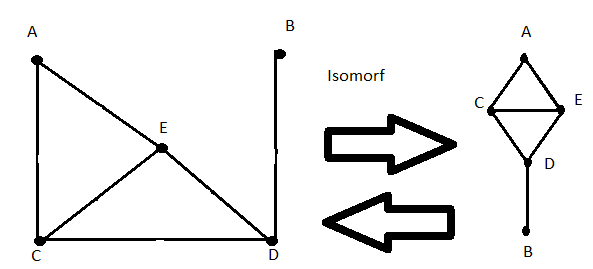
\includegraphics[scale=0.8]{grafteori1} \newline
		\textit{Figur 5.1: Isomorfe modeller}\newline
	\end{center}
	\vspace{-20pt}
	\vspace{-20pt}
\end{wrapfigure}

Denne matematik-type er stadig under udforskning, da der endnu ikke er en fuldstændig løsning på problemer i teorien, for blandt andet ”Traveling salesman problem”. Heriblandt findes mange typer af problemer, hvor forskellige teoretiske løsninger kan bruges. 
En af problematikkerne vedrørende Traveling salesman problem er,
at der ønskes både en optimal rute, og en en hensigtsmæssig udregningstid. Dette problem opstår i det, at en optimal rute skal findes mellem et hvis antal byer (knuder), hvor man i ét kan lave en hurtig estimeret ”kort” rute, hvis man starter med at lave tilfældige kanter fra knuderne, dog ikke mere end to kanter per knude, og derefter tester for, hvorvidt to nye kanter er kortere end to eksisterende kanter. På et tidspunkt vil en semi-optimal rute findes, dog er denne ikke nødvendigvis den fuldt optimale rute. Dette skyldes, at der igennem forløbet med udskiftning af kanter muligvis er truffet valg om rute som fører til, at en kortere kant ikke kan findes lokalt, men at den sammenlagte rute stadig ikke er optimal. Hvis der er fundet korte kanter lokalt, kan dette stoppe søgen i en kortere kant, da den korteste lokale kant er fundet, men ikke den korteste kant, hvis der tages hensyn til den sammenlagte kant-værdi. \citep{TSP} \newline

\textbf{Nearest neighbor algoritme}\newline
En af disse løsninger er Nearest neighbor algoritme, som behandler et problem der opstår, når en række knuder skal indgå, og kun skal indgå én gang, hvilket betyder, at der ikke må være en løkke (loop). Dette opnåes gennem brug af Hamiltonian Paths, hvilket er en ”rute” gennem knuder på grafen. I NNA vil en kant have en værdi, og disse værdier er bestemmende for, hvilken kant der skal følges. Fra den knude der behandles, skal kanten med den laveste værdi følges. Dette kan dog optimeres, ved at lave en matrice over kanterne fra alle knuder. Her tages højde for hvilke kanter der samlet set giver den korteste rute, uden brug af løkker. \citep{NNA}
\newline


\begin{wrapfigure}{}{0.4\textwidth}
	\vspace{-40pt}
	\begin{center}
		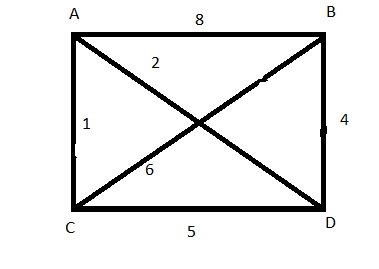
\includegraphics[scale=0.8]{grafteori2} \newline
		\textit{ Figur 5.2: Hamiltonian Path. \newline Følger kanter med laveste værdier.}
	\end{center}
	\vspace{-10pt}
\end{wrapfigure}

I dette tilfælde (figur 5.2), er den endelige rutes længde: 1+5+4+8 = 18. Spørgsmålet er så, er dette den koreste rute? Herefter opstilles en matrix, der beskriver alle kanter.

\begin{tabular}{| l | l | l | l | l | l |}
	\hline
	& A & B & C & D & E \\ \hline
	A & - & 3 & 1 & - & 2 \\ \hline
	B & 3 & - & - & 3 & 8 \\ \hline
	C & 1 & - & - & 5 & 6 \\ \hline
	D & - & 4 & 5 & - & 7 \\ \hline
	E & 2 & 8 & 6 & 7 & - \\
	\hline
\end{tabular}\newline


De mulige ruter er: \newline
ABDCE = 3+4+5+6 = 18. \newline
ACDBE = 1+5+4+8 = 18. \newline
AEBDC = 2+8+4+5 = 19. \newline
ABECD = 3+8+6+5 = 22. \newline
ABEDC = 3+8+7+5 = 23. \newline
ACEBD = 1+6+8+4 = 19. \newline
ACEDB = 1+6+7+4 = 18. \newline
AECDB = 2+6+5+4 = 17. \newline

Den korteste rute er altså AECDB, hvilket er 1 kortere end den antagede rute. Den optimale Hamiltonian Path er derfor denne rute. Dette tager NNA ikke højde for, da den starter i en valgt start-knude, og derefter følger kanten, med den derfra laveste værdi. Det smarte ved NNA er, at den ikke kræver meget kraft for en computer at udføre, hvorimod at finde den optimale Hamiltonian rute, vil være langt mere compliceret. NNA tager dog ikke højde for, hvad konsekvenser de skridt den tager, har for det endelige resultat.

\textbf{Dijkstra's algoritme}\newline
Udover NNA, findes også Dijkstra’s algoritme, hvor første step er, at bestemme ende-knuden, og sætte dens distance til nul. Denne knude sættes til at være den første knude, som behandles. I det en knude er checket færdig, vil denne knude markeres som ”besøgt”, og kanten med den mindste værdi følges, og næste knude markeres som ”nuværende” knude. En kant bliver kun fulgt, hvis det er den korteste rute, tilregnet tidligere kanter.
Problematikken med Dijkstra’s algoritme i forhold til dette projekt er, at den checker den korteste rute fra start-knude til slut-knude, men den indkluderer ikke nødvendigvis alle knuder som oplyses. I det denne rapport er afgrænset til fugleflugtslinjer, vil Dijkstra’s ikke være den optimale. Hvis en rute igennem en by, hvor der er tilregnet veje, stier og andre knuder, vil Dijkstra’s være det bedste valg. Denne algoritme vil også være i brug ved den optimale løsning. Ved brug af Dijkstra’s algoritme, vil den nuværende rute altid blive testet for, hvorvidt ruten der undersøges efter, er kortere eller længere end den hidtil korteste rute. Hvis den er kortere, vil denne rute blive sat som den hidtil korteste rute. \citep{Dijkstra}

/textbf{Double Minimum Spanning Tree}
Double Minimum Spanning Tree er algoritmen der ligger til grund for Christofides algoritme, hvor DMST hart re steps: Først oprettes et minimal spanning tree, som indkluderer alle knuder, hvorefter alle kanter duplikeres, og så skal den korteste rute findes mellem disse kanter, hvor en knude kun besøges én gang. Hvis ikke der er ubrugte kanter, oprettes en ”genvej” fra den nuværende knude til en ubesøgt knude \citep{DMST}. Denne metode kræver flere kræfter at køre end NNA, da NNA er en ringere algoritme til at finde den korteste rute, men dette projekt forholder sig til at finde en relativ kort rute, hvoraf en interessant rute kan findes.



\subsection{Vektorteori}
Essensen i dette projekt er at finde en flerpunktsrute mellem nogle valgte attraktioner, hvor brugeren skal have mulighed for, at vælge nogle attraktioner til deres rute. Gruppen vil ikke diktere hvad en interessant rute er for brugeren, derfor skal de have muligheden for at vælge de foreslåede attraktioner til eller fra.

\begin{wrapfigure}{}{0.4\textwidth}
	\vspace{-10pt}
	\begin{center}
		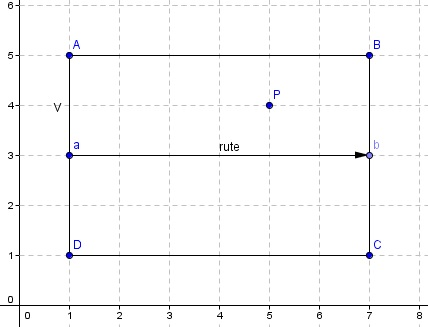
\includegraphics[scale=0.6]{matematikteori1} \newline
		\textit{Figur 5.1: Eksempel på om en attraktion er indenfor punkt a og b.}\newline
	\end{center}
	\vspace{-20pt}
\end{wrapfigure}

Der tages nu udgangspunkt i figur 5.1. En del af brugerens rute ligger fra attraktion a til attraktion b. Der skal nu tjekkes om der ligger andre attraktioner mellem afstanden fra a til b (eller AB), og med bredden AD hvor brugeren vil blive spurgt om denne attraktion skal tilføjes til ruten. AD er i projektets program sat til at være V * 2. Dette vil blive udregnet vha. vektorer 
Hvis der antages at punktet P er en attraktion som programmet skal tjekke, ligger denne inden for længden af ruten AB og bredden AD. Dette tjekkes med følgende formel:
\[0 < AP \cdot AB < AB \cdot AB \wedge 0 < AP \cdot AD < AD \cdot AD \]
Hvor prikproduktet af vektorerne AP og AB, skal være større end 0 og mindre end prikproduktet af vektorerne AB og AB. Det samme vil gælde for AD i stedet for AB.

Lad nu som om det de informationer der kendes er punkterne a og b, samt længden på vektor ab som vil være 6 og vektoren vil hedde:
\[ \begin{bmatrix} 6 \\ 0 \end{bmatrix} \]

Først ønskes punktet A findes, som gøres ved først at finde tværvektoren. Tværvektoren findes ved at bytte 1. og 2. koordinat rund og ændre fortegn på første koordinaten:
\[ \begin{matrix} a1 \\ a2 \end{matrix} = \begin{matrix} -a2 \\ a1 \end{matrix} \]
Tværvektoren hedder: 
\[ \begin{bmatrix} 6 \\ 0 \end{bmatrix} \text{ ,} \]
og har udgangs punkt fra punktet a. \newline
I dette eksempel skal der søges efter ekstra attraktioner langs ruten, svarende til 1/3 af rutens længde. Så for at finde koordinaterne til punktet A, finder vi først en enhedsvektor for tværvektoren, dette gøres med formlen:
\[ \overrightarrow{e} = \frac{1}{\overrightarrow{a}}*\overrightarrow{a} \] 

Dette giver en vektor: 
\[\ \begin{bmatrix} 0 \\ 1 \end{bmatrix} \text{ ,} \]
som også har udgangspunkt fra punktet a. Som tidligere nævnt søges der efter ekstra attraktioner langs ruten, svarende til 1/3 af rutens længde, så enhedsvektoren multipliceres med to, hvilket giver en vektor: 
\[\ \begin{bmatrix} 0 \\ 2 \end{bmatrix} \textbf{ .} \]
Denne vektor lægges til koordinaterne til punktet a, hvilket vil give punktet:
\[\ A = \begin{bmatrix} 1 \\ 3 \end{bmatrix} + \begin{bmatrix} 0 \\ 2 \end{bmatrix} = \begin{bmatrix} 1 \\ 5 \end{bmatrix} \text{ .} \]

Punktet D vil så ledes findes  ved at tage vektoren fra før og multiplicere med -2 og lægge punktet A til:
\[\ D = \begin{bmatrix} 0 \\ 2 \end{bmatrix} * -2 = \begin{bmatrix} 0 \\ -4 \end{bmatrix} + \begin{bmatrix} 1 \\ 5 \end{bmatrix} = \begin{bmatrix} 1 \\ 1 \end{bmatrix} \text{ .} \]



Dog vil der først findes en vektor AP mellem punkterne A og P med formlen: \[ \overrightarrow{AP} = \begin{matrix}X2-X1 \\ Y2-Y1\end{matrix} \]
Vektor AP: A(1,5) og P(5,4): \[ \overrightarrow{AP} = \begin{bmatrix}5-1 \\ 4-5\end{bmatrix} = \begin{bmatrix} 4 \\ -1 \end{bmatrix} \]
\[ \text{Vektor AB er allerede kendt, da det er det samme som } \overrightarrow{ab} \text{.} \]
For at projektere AP på AB skal følgende formel benyttes: \citep{ProjektionAfVektor} \[ b_{a} = (\frac{a*b}{|a|^2}) * a \]
Med denne formel vil vektoren b blive projekteret på vektoren a. I tælleren findes prikproduktet som kan findes ved at: \[ a \cdot b = \begin{matrix}X1 * X2 \\ Y1 * Y2\end{matrix}  \]
I nævneren findes længden på vektor a i anden, som kan regnes ved at sige: \[ \sqrt{ax^2+ay^2}^2 \]
Hvis der forsat tages udgangspunkt i eksemplet med figur 5.1, vil projektionen af AP på AB se således ud:
Prikproduktet af vektorerne: \[ \overrightarrow{AP} \cdot \overrightarrow{AB} = \begin{bmatrix} 4 & 6 \\ -1 & 0 \end{bmatrix} = 4*6+(-1)*0 = 24 \]
Længden af AB opløftet i anden vil være: \[ \sqrt{6^2+0^2}^2 = 36 \]
Ud fra dette kan vektoren fra projektionen af AP på AB findes: 
\[ \frac{24}{36} * \begin{bmatrix} 6 \\ 0 \end{bmatrix} \rightarrow \frac{24}{36} * 6 \wedge \frac{24}{36} * 0 = \begin{bmatrix} 4 \\ 0 \end{bmatrix} \]

Hvor resultatet vil give en ny vektor: \[ \begin{bmatrix} 4 \\ 0 \end{bmatrix} \text{ ,} \]  som også vil have startpunkt i A. Hvis der igen tages udgangspunkt i formlen:\newline
\begin{wrapfigure}{r}{0.4\textwidth}
	\vspace{-20pt}
	\begin{center}
		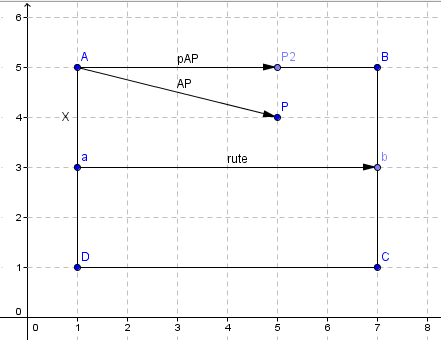
\includegraphics[scale=0.6]{matematikteori2} \newline
		\textit{Figur 5.2: Fortsat eksempel på om en attraktion er indenfor punkt a og b.}\newline
	\end{center}
	\vspace{-20pt}
\end{wrapfigure}
\[0 < AP \cdot AB < AB \cdot AB \wedge 0 < AP \cdot AD < AD \cdot AD \]
overholder punktet P første del, og ovenstående metode skal derfor gentages med vektoren AD i stedet for AB, for matematisk at finde ud af om punktet ligger inden 	for den afsatte bredde og længden af ruten a til b. Ved udregning af projektionen af AP på AD vil den nye vektor hedde: \[ \begin{bmatrix} 0 \\ -1 \end{bmatrix} \text{ .} \]\newline

\textbf{Opsummering}\newline
I grafteorien blev der konkluderet, at Nearest Neighbor algoritmen er den mest egnede til programmet, da dette projekt forholder sig til udregning af en relativt kort rute, hvorved en interessant rute kan findes efterfølgende. Vektorteorien gjorde grund for udregning af, hvilke attraktioner der er nærliggende, så en interessant rute kan findes ud fra ruten der i første omgang bliver dannet af NNA.

